\section{WIMP-nucleon interactions} \label{sec:wimp_nucleus_interactions}
\iffalse
\par
As WIMPs travel at relative non-relativistic speeds, the recoil energy of the nucleon resulting from an elastic scatter is by only the centre of mass scattering angle, $\theta$ \cite{direct_detection_of_wimps_ref}:
\begin{equation}
    E_{R} = \frac{{\mu}_{N}^{2}\nu_{\chi}^2}{m_{N}}(1-\cos(\theta))
\end{equation}
\fi
Direct dark matter detectors are built on the principle of having a large mass of material on which a WIMP can scatter \cite{direct_detection_of_wimps_ref}.
Within a detector, the rate of these WIMP scatter interactions, $R$, is given by:
\begin{equation}
    R = \sigma N_{T} n_{\chi} \langle v \rangle
    \label{eq:wimp_nucleon_rate}
\end{equation}
where N$_{T}$ is the number of nuclei in the detector, $n_\chi$ is the number density of dark matter particles travelling with an average speed $\langle v \rangle$ relative to the target, and $\sigma$ is the interaction cross-section, which represents the interaction strength between the dark matter and the nucleus.
\par
Given that each direct detector is sensitive to different recoil energies depending upon the design, it is beneficial to describe the event rate in an energy region as the differential scattering rate with respect to recoil energy \cite{supersymetry_wimpy_boi_ref}:
\begin{equation}
\begin{split}
    \frac{dR}{dE_R} &= \frac{\rho_{\chi}}{m_\chi m_A} \int^{\infty}_{v_{min}} v f(\vec{v}) \frac{d\sigma}{dE_R} d\vec{v} \\
                    &= \frac{2\rho_{\chi}}{m_\chi} \int^{\infty}_{v_{min}} v f(\vec{v}) \frac{d\sigma}{d |q|^2} d\vec{v}
\end{split}
\label{eq:wimp_differential_rate}
\end{equation}
where $f(\vec{v})$ is the dark matter velocity distribution in the galactic halo, $\rho_{\chi}$ is the dark matter density, $m_\chi$ is the dark matter mass, $m_A$ is the target nucleus mass, $q$ is the momentum transfer associated with the recoil given by $q = \sqrt{2m_A E_R}$ and $v_{min}$ is the minimum velocity of dark matter to induce a recoil of energy $E_R$.
It is a detector specific limit given by $v_{min} = \sqrt{(m_\chi E_R)/(2\mu^2)}$ where $\mu = (m_\chi m_A)/(m_\chi + m_A)$, the WIMP-nucleus reduced mass.
\par
We are able to control the detector size and target properties (within reason).
This leaves us with two parameters outside of our direct control but which we need to constrain in order to determine an expected rate of recoils in any given detector: the dark matter distribution and the differential cross-section.

\subsection{Local Astrophysical Dark Matter Properties}
\par
The standard dark matter model has two parameters that need to be determined experimentally: the velocity distribution and the density. 
Both have sufficient uncertainties which can significantly impact the sensitivity of any direct detection experiment \cite{local_dm_uncertainties_ref}.
\par
The local dark matter density has long been studied, with the earliest references from 1922 \cite{first_dm_density_1_ref, first_dm_density_2_ref}.
Since then, many measurements have been done which constrain $\rho_{\chi}$.
These fall into two categories: galactic measurements and local measurements \cite{dm_density_ref}.
Galactic measurements derive $\rho_{\chi}$ from rotation curves, which does not require the assumption of a galactic halo.
Local measurements typically observe tracer star motion near the Sun \cite{gaia_tracer_dm_density_ref}.
Naturally, there is variation in these two approaches where the galactic measurements place $\rho_{\chi}$ in the range 0.2-0.6 GeV/cm$^3$ whilst the latest result from Gaia \cite{gaia_data_2_ref} place $\rho_{\chi}$ between 0.1-1.5 GeV/cm$^3$ \cite{gaia_dm_density_2_ref}.
Before the second data release of Gaia, the best fit of all the studies lay in the range 0.22-0.33 GeV/cm$^3$, as such $\rho_{\chi}$ has typically been taken to be 0.3 GeV/cm$^3$.
This may change in the coming years as the current best fit from Gaia suggest $\rho_{\chi}=0.5$ GeV/cm$^{3}$ \cite{gaia_dm_density_1_ref}.
\par
With regard to the velocity distribution, there are a number of models that are often used. 
Including simple isotropic models \cite{isotropic_dark_matter_models_ref}, isothermal sphere dark matter \cite{dm_velocity_isothermal_ref} and the Standard Halo Model (SHM) \cite{dm_velocity_shm_ref}. 
We shall only consider the SHM here as it is the most common choice \cite{dark_matter_distribution_models_ref}.
\par
In the SHM, a Maxwell-Boltzmann velocity distribution is assumed, which is truncated at the escape velocity ($v_{\text{esc}}$) of the Milky Way \cite{direct_dark_matter_of_wimps_concepts_ref}.
This constrains the dark matter to be within the galaxy.
The SHM also assumes dark matter is isotropic and spherically symmetrically distributed in the galaxy\footnote{The distribution is not perfectly symmetrical, and there are newer models referred to as SHM$^{++}$ which try and account for this, but they are not considered here \cite{extended_shm_ref}}.
The velocity distribution of dark matter within the Milky Way halo in the Earth frame is approximated as \cite{direct_dark_matter_of_wimps_concepts_ref, shm_derivation_ref}:
\begin{equation}
    f(\vec{v}) = \frac{1}{k} e^{\frac{- (\vec{v} - \vec{v}_E)^2 }{ v^2_0} }
    \label{eq:shm_short_equation}
\end{equation}
where $\vec{v}$ is the velocity of the dark matter with respect to the Earth, $\vec{v}_E$ is the velocity of the Earth around the centre of the galaxy and $\vec{v}_0$ is the peculiar velocity of the Sun relative to its circular velocity. 
\autoref{eq:shm_short_equation} is only valid for when $|\vec{v} + \vec{v}_E| < v_{\text{esc}}$.


%\begin{equation}
% f(\vec{v}) = \frac{1}{(2\pi\sigma^2_{v})^{\frac{3}{2}}N_{esc}} e^{\frac{- |\vec{v}|^2}{2\sigma^2_v}} \Theta(v_{esc} - |\vec{v}|)
%\label{eq:shm_velocity_1}
%\end{equation}
%where $\Theta$ is a Heaviside step function, $\sigma_v$ is the velocity dispersion, and .
%
%\par
%The dark matter velocity distribution which was used in \autoref{eq:wimp_differential_rate_scattering_amplitude} was normalised such that $\int f(\vec{v}) dv = 1$.
%As such we need to renormalise \autoref{eq:shm_velocity_1} to allow for the integral of $\sigma_{v}$ to be unitary as well.
%We do this by:
%\begin{equation}
%    N_{esc} = erf(z) - 2z e^\frac{-z^2}{\pi^{\frac{1}{2}}}
%\end{equation}
%where erf is the error function (given by $\text{erf}(z) = 2/\sqrt{\pi}\int^{z}_{0} e^{-t^2} dt$) and $z=v_{esc}/v_0$.
%We also need to define two other variables: $x=v_{min}/v_{0}$ and $y=|V_E|/v_0$ where $|V_E|$ is the velocity of the Earth with respect to the dark matter halo.
%Using these we can define our integral as \cite{shm_derivation_ref}:
%\begin{equation}
%\begin{split}
% \int \frac{f(\vec{v})}{v} = 
%\begin{dcases}
%\frac{1}{v_0 y}  & \text{if}\; z<y,x<|y-z| \\
%\frac{1}{2N_{esc} v_{0}y} \bigg[\text{erf}(x+y) - \text{erf}(x-y) - \frac{4}{\sqrt{\pi}}ye^{-z^2} \bigg] & \text{if}\; z>y, x<|y-z| \\
%\frac{1}{2N_{esc} v_{0}y} \bigg[\text{erf}(z) - \text{erf}(x-y) - \frac{2}{\sqrt{\pi}}(y + z - x)e^{-z^2} \bigg] & \text{if}\; |y-z|<x<|y+z|
%\end{dcases}
%\end{split}
%\label{eq:shm_velocity_2}
%\end{equation}
\par
Depending upon the values used for both the dark matter density and the velocities, the scattering rate will vary, and therefore the sensitivity of any given experiment will vary.
Historically the parameters used for determining the event rate have varied between experiments, making comparisons between results difficult.
A recent collaboration between direct dark matter experiments has led to an agreed-upon common set of parameters \cite{standard_halo_model_conventions_ref}, which are summarised in \autoref{tab:standard_parameters_for_dm}.
For a review of how these affect sensitivity to a dark matter discovery, the reader is directed to \cite{dm_velocity_effects_on_limits_ref}.

\begin{table}[]
    \centering
    \begin{tabular}{c|c|c}
        Parameter                               & Description                       & Value         \\ \hline
        $\rho_{\chi}$                           & Local dark matter density         & 0.3 GeV/cm$^2$ \cite{shm_derivation_ref}           \\
        $v_{esc}$                             & Galactic escape velocity          & 544 km/s  \cite{dm_v_esc_ref}           \\
        $v_0$                             & Local standard of rest velocity   & 238 km/s   \cite{dm_v_0_ref}           
    \end{tabular}
    \caption{Suggested Standard Halo Model parameters adapted from \cite{standard_halo_model_conventions_ref}}
    \label{tab:standard_parameters_for_dm}
\end{table}

\subsection{Differential cross-section}
\par
As has already been said, we are constraining ourselves to non-relativistic scattering.
Therefore only interactions which do not vanish in the zero-momentum transfer limit need to be considered, of which there are two: a spin-independent (SI) and a spin-dependent (SD) component \cite{wimp_lagrangian_ref}.
The differential cross-section is then given by:
\begin{equation}
    \frac{d\sigma}{d|q|^2} = \bigg(\frac{d\sigma}{d|q|^2}\bigg)_{SI} + \bigg(\frac{d\sigma}{d|q|^2}\bigg)_{SD}
\end{equation}
The SI interaction arises from the WIMP coupling to quarks mediated via a Higgs, whereas SD interactions arise from the axial-vector interaction between WIMPs and quarks \cite{supersymmetric_dark_matter_ref}.
As the weighted contributions of the SI and SD components are not known and to make experimentalists lives easier, each interaction is generally considered independently, but for those interested in mixing these terms, the interaction Lagrangian can be found in \cite{wimp_lagrangian_ref}.
%, following \cite{supersymetry_wimpy_again_ref}.
\par
In this zero-momentum transfer regime, the WIMP-nucleus cross-section can be expressed as:
\begin{equation}
    \frac{d\sigma}{d|q|^2} = \frac{\sigma_0}{4\mu^2 v^2} F^2(q)
\end{equation}
where $\sigma_0$ is the total cross-section at zero-momentum transfer and $F(q)$ is the nuclear form factor that encapsulates the momentum dependence of the cross-section \cite{shaunalsum_thesis_ref}.
This identity is known as Fermi's Golden rule \cite{shaunalsum_thesis_ref}.
\par
Taking the SI case only, and so setting the contribution from SD to zero, the WIMP-nucleus cross-section is \cite{supersymetry_wimpy_again_ref}:
\begin{equation}
    \sigma_0 = \frac{4\mu^2}{\pi} [f_pZ + f_n (A-Z)]^2
\end{equation}
where $A$ and $Z$ are the atomic mass and atomic number, respectively.
$f_n$ and $f_p$ are the dark matter couplings to neutrons and protons.
\par
If we assume that the coupling for WIMPs to protons and neutrons is similar\footnote{so isospin is conserved} ($f_p \backsim f_n$) then the relation between the WIMP-nucleus and WIMP-nucleon cross-sections is given by \cite{wimp_sd_form_factor_ref}:
\begin{equation}
    \sigma_{0} = \frac{\mu^2}{\mu^2_n}A^2 \sigma_{n}
\end{equation}
where $\mu_n$ is the WIMP-nucleon reduced mass and $\sigma_n$ is the WIMP-nucleon cross-section.
\par
The final WIMP-nucleon elastic scattering differential rate for an SI interaction is then given by \cite{wimp_theory_ref}:
\begin{equation}
    \frac{dR}{dE_R} = \frac{\rho_\chi}{2 m_\chi \mu^2} F^2(q) \int^{\infty}_{v_{min}} \frac{f(\vec{v})}{v} A^2 \sigma_{0n} d\vec{v}
    \label{eq:wimp_si_differential_rate}
\end{equation}
An equivalent derivation for SD interactions can be found in \cite{wimp_theory_ref}.
It is typical to report any result in terms of WIMP-nucleon cross-section as it removes the dependence on the target nuclei, allowing different experiments to compare results easily.

\par
In the left plot of \autoref{fig:si_recoil_and_form_factor}, the differential event rate for a selection of frequently used targets is shown.
In \autoref{fig:si_recoil_and_form_factor}, a WIMP mass of 100 GeV/c$^2$ is used with a WIMP-nucleon cross-section of 10$^{-45}$ cm$^2$ (i.e. 1 zb).
Results from experiments are typically normalised to a cross-section of 1 zb to allow for easier comparison.
The heavy target nuclei have a larger event rate for low-energy nuclear recoils.
This is due to the A$^2$ enhancement seen in \autoref{eq:wimp_si_differential_rate}.
A lower scattering rate is seen for lighter nuclei, but at higher recoil energies, they have a higher rate than heavy nuclei.
This is due to a rate suppression by the form factors (discussed in the next section) and a decrease in kinematically-allowed WIMP velocities with an increase in $m_A$ and $E_R$.

\begin{figure}
    \centering
    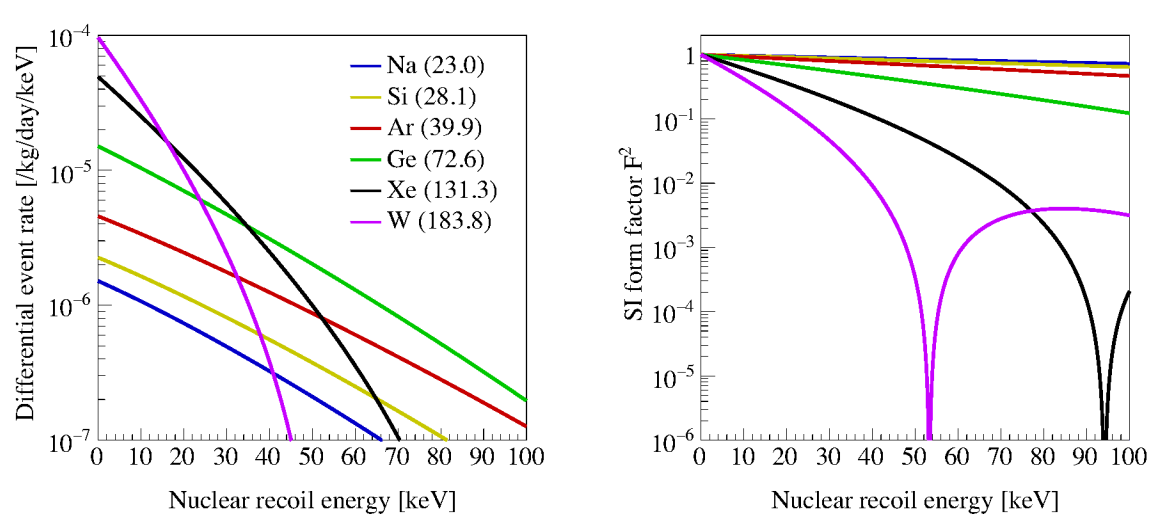
\includegraphics[width=\textwidth]{Figures/LZ/SI_recoil_rate_and_spectra.png}
    \caption{\textbf{Left:} SI nuclear recoil rate for a selection of target elements for a WIMP mass of 100 GeV/c$^2$ and WIMP-nucleon cross-section of $\sigma_N=$1 zb and the recommended parameters for the SHM. The averaged atomic mass of each target from natural abundance is in the brackets.
    \textbf{Right:} The Helm form factors for a selection of target nuclei. The key is the same in both plots.
    Both plots are from \cite{LZ_Ibles_LZStats_Thesis_ref}
    \label{fig:si_recoil_and_form_factor}.
           }
\end{figure}
 
\subsection{Form Factors}
\label{sec:form_factors}
\par
One feature which hasn't been mentioned in detail yet is the form factor, $F(q)$.
The form factor contains the physics of the nucleus and is the Fourier transform of the density distribution within.
For SI interactions, this is taken to be the Helm form factor where the nucleus is represented as a solid sphere of radius $r_n$, with a smooth density of nucleons described by a Gaussian of thickness $s$ \cite{helm_form_factor_ref}:
\begin{equation}
    F^2(q) = \bigg( \frac{3j_i(qr_n)}{qr_n} \bigg)^2 e^{-q^2 s^2}
\end{equation}
where $j_i$ is the Bessel function.
\par
%As $r_n \backsim A^{1/3}$ fm, we can see that the WIMP cannot resolve the nucleus as a point-like object.
In the right plot of \autoref{fig:si_recoil_and_form_factor}, the Helm form factors for a selection of popular targets are shown.

\par
For SD interactions, the coupling is not equal between protons and neutrons and so the choice of which nucleus description to use is fairly important.
Depending on which is used, the resultant sensitivity to dark matter can vary by orders of magnitude \cite{wimp_nuclear_model_ref,wimp_sd_form_factor_ref}.
